\chapter{Approksimationsalgoritmer}

\section{Set-Cover Problemet}%
\label{sec:SetCover}

\textsc{Set-Cover} problemet, siger, at givet et input $(X, \mathcal{F})$, hvor $X$ er en endelige mængde og $\mathcal{F}$ er en familie af delmængder af $X$, så find en delmængde $\mathcal{F}'$ af $\mathcal{F}$, således at $\bigcup_{S \in \mathcal{F}'} S = X$, hvor $|\mathcal{F}|$ er minimeret.

\begin{wrapfigure}{r}{0.5\textwidth}
  \centering
  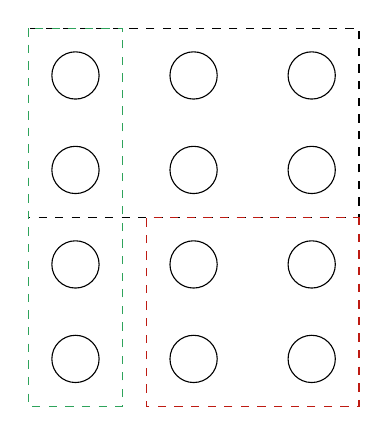
\begin{tikzpicture}[scale=1.2]
    \draw  (7.25,15) circle (0.25cm);
    \draw  (7.25,14) circle (0.25cm);
    \draw  (7.25,13) circle (0.25cm);
    \draw  (7.25,12) circle (0.25cm);
    \draw  (8.5,15) circle (0.25cm);
    \draw  (8.5,14) circle (0.25cm);
    \draw  (8.5,13) circle (0.25cm);
    \draw  (8.5,12) circle (0.25cm);
    \draw  (9.75,15) circle (0.25cm);
    \draw  (9.75,14) circle (0.25cm);
    \draw  (9.75,13) circle (0.25cm);
    \draw  (9.75,12) circle (0.25cm);
    \draw [, dashed] (6.75,15.5) rectangle  (10.25,13.5);
    \draw [ color={rgb,255:red,46; green,163; blue,91} , dashed] (6.75,15.5) rectangle  (7.75,11.5);
    \draw [ color={rgb,255:red,190; green,27; blue,19} , dashed] (10.25,13.5) rectangle  (8,11.5);
  \end{tikzpicture}
  \caption{\label{fig:setcover} Et eksempel på en løsning af et Setcover Problem hvor $|\mathcal{F}'| = 3$}
\end{wrapfigure}

I Figur~\ref{fig:setcover} ses et eksempel på en løsning af en instans af set-cover problemet, hvor $|\mathcal{F}'| = 3$. Bemærk dog at delmængderne i $\mathcal{F}'$ ikke behøver at have den form, de skal bare være normale delmængder.

Optimiseringsversionen af \textsc{Vertex-Cover} er et specielt case af \textsc{Set-Cover}, hvilket betyder, at når vi ved at \textsc{Vertex-Cover} problemet er svært at løse, så er \textsc{Set-Cover} også. Vi transformerer fra \textsc{VC} til \textsc{SC} som følger: Givet en graf $G = (V,E)$, konstruer en instans $(X, \mathcal{F})$ af \textsc{Set-Cover} problemet. Lad $X = E$ og $\mathcal{F} = \{S_{v} \mid v \in V\}$, hvor $S_{v}$ er mængden af kanter som $v$ ``dækker''. Dette er en reduktion, så dermed, siden decision versionen af \textsc{Vertex-Cover} er NP-komplet, så er decision versionen af \textsc{Set-Cover}, som tager en instans $(X, \mathcal{F}, k)$ og spørger om det er muligt at ``dækker'' alle mængder med højest $k$ delmængder. delmængder.

I Algoritme~\ref{alg:greedysetcover} ses en grådig algoritme som finder et cover. I algoritmen er variablen $Z$ de elementer der endnu ikke er dækket, og $\mathcal{F}'$ er delmængderne som dækker den del af $X$ der er dækket, altså $\overline{Z}$. Løkken vælger en delmængde i $\mathcal{F}$ som dækker flest mulige nye elementer. Bemærk dog, at algoritmen antager at det er muligt at dækker alle elementer i $X$, altså $\bigcup_{s \in \mathcal{F}} s = X$.

\begin{algorithm}
\caption{\label{alg:greedysetcover}Grådig Set Cover}
\begin{algorithmic}
\REQUIRE $X$, $\mathcal{F}$
\STATE $Z \leftarrow X$
\STATE $\mathcal{F}' \leftarrow \emptyset$
\WHILE{$Z \neq \emptyset$}
    \STATE Vælg $S \in \mathcal{F}$ således at $|S \cap Z|$ er maksimeret.
    \STATE $Z \leftarrow Z \setminus S$
    \STATE $\mathcal{F}' \leftarrow \mathcal{F}' \cup \{S\}$
\ENDWHILE
\RETURN $\mathcal{F}'$
\end{algorithmic}
\end{algorithm}

\begin{theorem}
Den grådige set-cover algoritme er en $H(|X|)$-approksimationsalgoritme.
\end{theorem}
\begin{proof}
  Husk at $\sum_{i=1}^n \frac{1}{i} = H(n)$. Vi ser på mængden af delmængder vi vælger til set-coveret som værende $\mathcal{F}' = \{S_{1}, S_{2}, \ldots, S_{|\mathcal{F}'|}\}$, hvor $S_{|\mathcal{F}'|}$ er den sidste delmængde, og den der dækker de resterende elementer.

  $\forall x \in X$: Lad $S_{i}$ være den første mængde i $\mathcal{F}'$ som indeholder $x$ og tildel $x$ \textit{vægten} $c_{x} = \frac{1}{|S_{i} \setminus (S_{1} \cup \cdots \cup S_{i-1})|}$. Altså kan man se på vægten som værende $\frac{1}{x}$ hvor $x$ er antallet af nye elementer dækket af $S_{i}$. Dermed vil hvert element i en delmængde der dækker 10 nye elementer have vægt $\frac{1}{10}$. Hvis man summerer vægten for hvert element i grafen, får man antallet af delmængder i løsningen $\mathcal{F}'$. For eksempel, hvis en delmængde dækker 20 elementer i alt, og af disse 20 er 10 af elementerne ikke dækket får, så får hvert element vægt $\frac{1}{10}$ og når vi summerer den nydækkede del får vi $\frac{1}{10} \cdot 10 = 1$. Dermed får vi ligningen $|\mathcal{F}'| = \sum_{x \in X} c_{x}$.

  Vi vil nu estimere hvor langt fra det optimale vi er. Lad $\mathcal{F}^{*}$ være den optimale familie af delmængder.
  \begin{equation}
    \label{eq:flessthanoptimal}
    |\mathcal{F}'| = \sum_{x \in X}^n \le \sum_{S \in \mathcal{F}^{*}} \sum_{x \in S} c_{x}
  \end{equation}

  Uligheden i~\ref{eq:flessthanoptimal} kommer fra, at vi beholder værdien på hvert element, $c_{x}$; som nu muligvis er i mere end en delmængde fra $\mathcal{F}$. Dermed vil den muligvis også blive tællet mere end én gang.

  \begin{claim}
    \label{claim:costlessthanharmonic}
    \begin{equation*}
      \sum_{x \in S} c_{x} \le H(|S|) \forall S \in \mathcal{F}
    \end{equation*}
  \end{claim}
  Hvis vi antager påstand~\ref{claim:costlessthanharmonic} til at være korrekt, får vi følgende resultat:
  \begin{align*}
    |\mathcal{F}'| \le \sum_{s \in \mathcal{F}^{*}} \sum_{x \in S} c_{x} &\le \sum_{s \in \mathcal{F}^{*}} H(|S|)\\
                                         &\le \sum_{S \in \mathcal{F}^{*}} H(\max_{S \in \mathcal{F}} |S|) \\
                                         &\le \sum_{s \in \mathcal{F}^{*}} H(|X|)\\
                                         &= |\mathcal{F}^{*}| H(|X|)
  \end{align*}
  Dette viser at den grådige algoritme er en $H(|X|)$-approksimationsalgoritme.
\end{proof}

Vi vil nu bevise påstand~\ref{claim:costlessthanharmonic}.

\begin{proof}
  Vi kigger på en arbitrær fastsat $S \in \mathcal{F}$ og lader $k$ være en konstant således at $S \not \subseteq S_{1} \cup \cdots \cup S_{k-1}$ men $S \subseteq S_{1} \cup \cdots \cup S_{k}$.

  Lad $u_{i} = |S \setminus S_{1} \cup \cdots \cup S_{i}|$ for $i = 0,1, \ldots, k$. Altså kan $u_{i}$ defineres til at være antallet af elementer som endnu ikke er dækket af delmængderne $S_{1} \cup \cdots \cup S_{i}$. Ud fra denne definition er det klart at se at $u_{0} = |S|$, $u_{k} = 0$, og $u_{i-1} \ge u_{i}$. Vi kan ud fra dette også se at $u_{i-1} - u_{i}$ er antallet af nye elementer af $S$ som dækkes af $S_{i}$.
\end{proof}
%% 22:09

%%% Local Variables:
%%% mode: latex
%%% TeX-engine: xetex
%%% TeX-command-extra-options: "-shell-escape"
%%% TeX-master: "main"
%%% End:
